\section{Uniform Distribution}
\label{sec:Uniform density function}

\subsection{Objective}
Generate uniform random numbers and plot
their density function. Find the mean and variance.

\subsection{Theory}
The uniform distribution is a continuous probability distribution where all outcomes are equally likely.
It is defined by two parameters, a and b, which are the minimum and maximum values that the random variable can take.
The probability density function is given by:

\begin{equation}
    f(x) = \frac{1}{b-a} \quad \textnormal{ for } \quad a \leq x \leq b
\end{equation}

\subsection{Matlab Code}
\inputminted[fontsize=\footnotesize,autogobble]{matlab}{code/uniform.m}

\subsection{Output}

\begin{figure}[!htb]
    \centering
    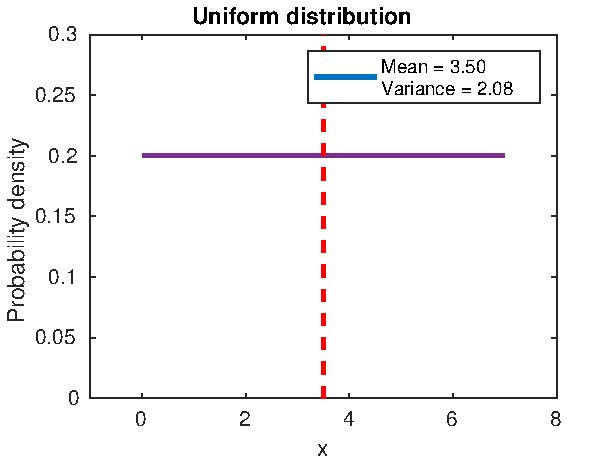
\includegraphics[width=0.6\textwidth]{res/figures/Figure_5.pdf}
    \label{output:uniform distribution}
    \caption{Uniform Distribution}
\end{figure}